\documentclass[10pt,twocolumn,letterpaper]{article}
\usepackage[margin=0.75in,columnsep=0.3in]{geometry}
\usepackage{times}
\usepackage{amsmath,amssymb}
\usepackage{graphicx}
\usepackage{booktabs}
\usepackage{multirow}
\usepackage{xcolor}
\usepackage{tikz}
\usetikzlibrary{arrows.meta,positioning,fit,backgrounds,calc}
\usepackage[numbers,sort&compress]{natbib}
\usepackage[colorlinks=true,linkcolor=blue,citecolor=blue,urlcolor=blue]{hyperref}
\usepackage[capitalise,nameinlink]{cleveref}

\graphicspath{{figures/}}

\newcommand{\etal}{et~al.}
\newcommand{\vs}{vs.}
\newcommand{\todo}[1]{\textcolor{red}{[TODO: #1]}}
\newcommand{\best}[1]{\textbf{#1}}
\newcommand{\std}[1]{{\scriptsize$\pm$#1}}

% Coverage and negative-pair numbers (proj/scripts/paper_analysis.py, 50 MegaDepth pairs, seed-0 policy)
\newcommand{\COVov}{7.6}\newcommand{\COVog}{\best{12.3}}\newcommand{\COVor}{9.7}
\newcommand{\COVbv}{10.6}\newcommand{\COVbg}{\best{17.0}}\newcommand{\COVbr}{14.6}
\newcommand{\COVTEXT}{more of the image: for ORB, 12.3\,\% of the $16{\times}16$ cells contain a RANSAC
inlier, against 7.6\,\% for vanilla and 9.7\,\% for RIPE-Select (BRISK: 17.0, 10.6 and 14.6\,\%)}
\newcommand{\NEGTEXT}{We tested whether this explains the ORB result, on 50 MegaDepth pairs, each also
paired with an image of the other scene. The evidence does not support it. For ORB, RIPE-Select lowers
the mean number of RANSAC inliers on these negative pairs only from 21.8 to 19.5, the ratio of inliers
on positive to negative pairs is unchanged (7.0 \vs 7.1 for vanilla), and every ORB negative pair still
yields at least 15 inliers for every method. For BRISK the ratio does improve (8.4 \vs 6.2), but there
RL and supervised training perform the same. Why RL helps ORB therefore remains open. One untested
explanation is that RL learns from the matches among \emph{sampled} subsets of the pool, as at test
time, whereas the supervised labels are computed once on the full pool, where ORB's many
near-duplicate binary descriptors match differently.}

% Source notes for the next revision (not printed):
%  - MegaDepth uses 500 of the 1500 pairs; re-run with all pairs before submission (drop --limit in run_all.ps1).
%  - Update RL rows to 5 seeds once ORB/BRISK seeds 3 and 4 finish training.
%  - Optional: K-sweep (256-4096) of RL vs pool grid.

\title{Learning Which Classical Keypoints to Keep:\\Pair-Label Reinforcement for ORB and BRISK Selection}
\author{Krishnavamsi\\\todo{Affiliation}\\{\tt\small vamsi9398672280@gmail.com}}
\date{}

\begin{document}
\maketitle

% ---------------------------------------------------------------------------
\begin{abstract}
Classical binary features such as ORB and BRISK remain the default in SLAM, embedded vision and
licence-constrained pipelines, yet which of their candidates are kept is decided by a detector
response that barely predicts whether a keypoint will match. We ask whether the weak, pair-level reward
introduced by RIPE --- a match is rewarded if it survives epipolar RANSAC on an image pair of the same
scene and penalised on a pair of different scenes --- can teach a policy \emph{which} classical keypoints
to keep, leaving the detector, the descriptor and the matcher untouched. We train a small MLP over
per-candidate cues with REINFORCE, using a Bernoulli selection whose per-image bias enforces an exact
keypoint budget. Trained on two IMC-2020 scenes on a laptop CPU, the policy improves relative-pose AUC on
MegaDepth-1500 by \best{+8.8} (ORB) and \best{+4.7} (BRISK) mean AUC over OpenCV, averaged over three
seeds, and raises match precision and inlier ratio. Reinforcement learning matters for the binary ORB
descriptor, where it beats a supervised model trained on the same RANSAC pseudo-labels by +5.7 AUC.
We also report where learned selection does not help: a spatial-bucketing heuristic on the same
candidate pool reaches comparable pose accuracy, and on the planar HPatches benchmark no learned variant
beats it.
\end{abstract}

% ---------------------------------------------------------------------------
\section{Introduction}
\label{sec:intro}

Learned local features~\cite{detone2018superpoint,tyszkiewicz2020disk,zhao2023aliked,kunzel2025ripe}
now dominate image-matching benchmarks, but classical detectors and descriptors are still what many
deployed systems run: ORB~\cite{rublee2011orb} is the front end of ORB-SLAM~\cite{murartal2015orbslam},
and binary features are preferred wherever compute, memory or licensing are tight. These pipelines
detect many candidates and keep the $K$ with the highest detector response. Response measures local
contrast, not \emph{matchability}: on MegaDepth we find that it separates keypoints that later become
correct matches from those that do not with a ROC-AUC of only 0.56--0.60, and that a top-$K$ cut by
response discards more than half of the correct matches present in the candidate pool.

RIPE~\cite{kunzel2025ripe} recently showed that a keypoint detector can be trained with reinforcement
learning from nothing more than the knowledge of whether two images show the same scene. We transfer
this idea to classical features. A classical detector has no heatmap to sample from, so instead of
learning the detector we learn a \emph{selection policy} over its candidates (\cref{fig:pipeline}). The
detector, the descriptor, the matcher and the robust estimator stay exactly as they are; only the
decision of which $K$ keypoints are kept is learned. The result is a drop-in module for existing
pipelines.

\paragraph{Contributions.}
\begin{itemize}\setlength\itemsep{0pt}
  \item \textbf{RIPE-Select}, a keypoint selection policy for classical detectors trained with RIPE's
        pair-label reward, together with a budget-exact Bernoulli sampling scheme that replaces RIPE's
        keypoint-count regulariser (\cref{sec:method}).
  \item A controlled evaluation in which every compared method uses the same images, candidate pool,
        budget, descriptor, matcher and RANSAC, with three training seeds and paired bootstrap tests
        (\cref{sec:setup}).
  \item Evidence that the reward transfers: +8.8 and +4.7 mean pose AUC over OpenCV for ORB and BRISK on
        MegaDepth-1500, with higher match precision and inlier ratio (\cref{sec:results}).
  \item An analysis of when RL is needed and of what limits it: RL beats supervised training for the
        binary ORB descriptor but not for BRISK, the policy improves match quality but not spatial
        coverage, and selection does not help on planar scenes (\cref{sec:analysis}).
\end{itemize}

% ---------------------------------------------------------------------------
\begin{figure*}[t]
\centering
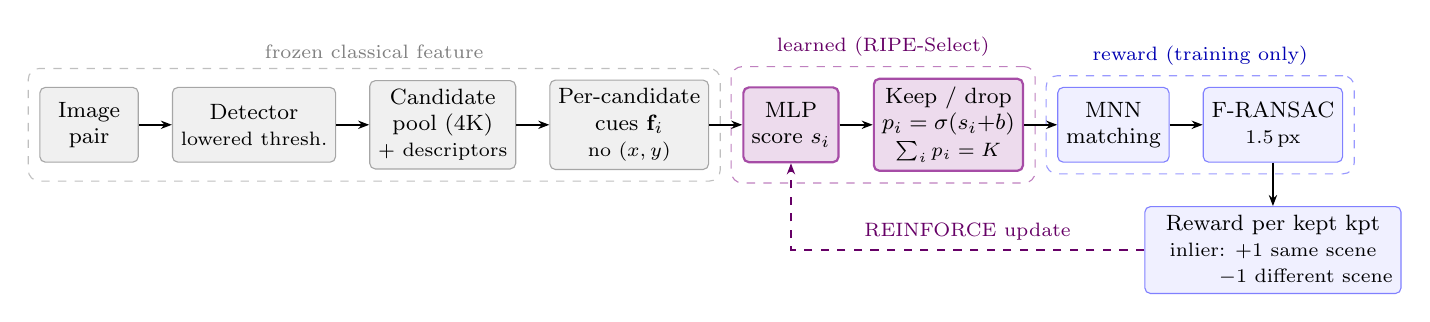
\begin{tikzpicture}[
    font=\footnotesize,
    box/.style={draw, rounded corners=2pt, align=center, minimum height=0.95cm, inner sep=3pt},
    frozen/.style={box, fill=gray!12, draw=gray!70},
    learned/.style={box, fill=violet!14, draw=violet!70, thick},
    eval/.style={box, fill=blue!6, draw=blue!50},
    arr/.style={-{Stealth[length=4pt]}, semithick},
    node distance=0.42cm]
  \node[frozen, minimum width=1.25cm] (img) {Image\\pair};
  \node[frozen, right=of img] (det) {Detector\\{\scriptsize lowered thresh.}};
  \node[frozen, right=of det] (pool) {Candidate\\pool (4K)\\{\scriptsize + descriptors}};
  \node[frozen, right=of pool] (cue) {Per-candidate\\cues $\mathbf{f}_i$\\{\scriptsize no $(x,y)$}};
  \node[learned, right=of cue] (mlp) {MLP\\score $s_i$};
  \node[learned, right=of mlp] (sel) {Keep / drop\\$p_i=\sigma(s_i{+}b)$\\{\scriptsize $\sum_i p_i = K$}};
  \node[eval, right=of sel] (mnn) {MNN\\matching};
  \node[eval, right=of mnn] (ran) {F-RANSAC\\{\scriptsize 1.5\,px}};
  \node[eval, below=0.55cm of ran, minimum width=2.2cm] (rew) {Reward per kept kpt\\
        {\scriptsize inlier: $+1$ same scene}\\{\scriptsize\phantom{inlier: }$-1$ different scene}};
  \foreach \a/\b in {img/det, det/pool, pool/cue, cue/mlp, mlp/sel, sel/mnn, mnn/ran, ran/rew}
    \draw[arr] (\a) -- (\b);
  \draw[arr, dashed, violet!80!black] (rew.west) -| node[pos=0.25, above, font=\scriptsize]
        {REINFORCE update} (mlp.south);
  \begin{scope}[on background layer]
    \node[draw=gray!50, dashed, rounded corners, fit=(img)(cue), inner sep=4pt,
          label={[font=\scriptsize, gray]above:frozen classical feature}] {};
    \node[draw=violet!50, dashed, rounded corners, fit=(mlp)(sel), inner sep=4pt,
          label={[font=\scriptsize, violet!80!black]above:learned (RIPE-Select)}] {};
    \node[draw=blue!40, dashed, rounded corners, fit=(mnn)(ran), inner sep=4pt,
          label={[font=\scriptsize, blue!70!black]above:reward (training only)}] {};
  \end{scope}
\end{tikzpicture}
\caption{\textbf{RIPE-Select.} The classical detector and descriptor are frozen (grey); only the choice
of which $K$ candidates are kept is learned (violet). During training, kept keypoints are matched and
rewarded if they survive RANSAC on a same-scene pair, and penalised if they survive on a different-scene
pair. At test time the $K$ highest-scoring candidates are kept and passed to the unchanged pipeline.}
\label{fig:pipeline}
\end{figure*}

\section{Related work}
\label{sec:related}

\paragraph{Classical detectors and descriptors.}
SIFT~\cite{lowe2004sift} detects scale-space extrema of a difference of Gaussians. ORB~\cite{rublee2011orb}
combines oriented FAST~\cite{rosten2006fast} corners, ranked by a Harris score, with a rotated BRIEF
descriptor. BRISK~\cite{leutenegger2011brisk} uses AGAST~\cite{mair2010agast} corners in scale space and
a 512-bit sampling-pattern descriptor. In all three, the number of keypoints is controlled by a
response threshold and a top-$K$ cut.

\paragraph{Keypoint selection and spatial distribution.}
Adaptive non-maximal suppression~\cite{brown2005anms} and its fast variants~\cite{bailo2018ssc} keep
strong keypoints that are far apart. ORB-SLAM~\cite{murartal2015orbslam} buckets keypoints into a grid
so that every cell contributes. These methods change \emph{where} keypoints are kept, not \emph{how
good} each one is; we include grid bucketing as a baseline.

\paragraph{Predicting matchability.}
Hartmann~\etal~\cite{hartmann2014matchability} train a classifier to discard SIFT keypoints that are
unlikely to match before matching, supervised by structure-from-motion tracks. We share the goal but
differ in supervision: our policy needs only pair labels, and it is trained directly on the outcome of
matching and RANSAC.

\paragraph{Learned detectors.}
SuperPoint~\cite{detone2018superpoint}, Key.Net~\cite{barroso2019keynet},
DISK~\cite{tyszkiewicz2020disk} and ALIKED~\cite{zhao2023aliked} learn detectors, mostly with depth,
pose or homography supervision. DISK and RIPE~\cite{kunzel2025ripe} use policy gradients; RIPE needs only
image-pair labels. These methods replace the whole feature; ours keeps the classical one.

% ---------------------------------------------------------------------------
\section{Method}
\label{sec:method}

\subsection{Candidate pool}
We run the unchanged OpenCV detector with lowered thresholds to obtain more candidates than the budget:
FAST threshold 7 with up to 8K points for ORB, and AGAST threshold 10 instead of 30 for BRISK. The pool
is cut to the $4K$ strongest candidates by response, and the unchanged OpenCV descriptor is computed for
every candidate.

\subsection{Per-candidate cues}
Each candidate $i$ is described by a vector $\mathbf{f}_i$ of 20 scalar cues followed by its descriptor
bits (276 inputs for ORB, 532 for BRISK). The cues cover the detector response and its rank, scale and
pyramid level, near-duplicate detections, local keypoint density and rank within the neighbourhood,
intra-image descriptor distinctiveness, and patch statistics at the keypoint scale; the full list is in
\cref{app:cues}. The image coordinates $(x,y)$ are deliberately \emph{not} given, so the policy cannot
learn scene-specific locations.

\subsection{Policy and budget-exact sampling}
A three-layer MLP (hidden sizes 128 and 64, ReLU) maps $\mathbf{f}_i$ to a score $s_i$. During training
each candidate is kept independently with probability
\begin{equation}
  p_i = \sigma(s_i + b), \qquad \textstyle\sum_i p_i = K,
  \label{eq:bias}
\end{equation}
where the bias $b$ is solved per image. Because $\sum_i p_i$ is monotone in $b$, it is found by
bisection. This fixes the expected number of kept keypoints to the budget, so the policy can only change
\emph{which} keypoints are kept, not how many. It replaces the keypoint-count regulariser used by RIPE,
which would otherwise let the policy trade quantity for quality. At test time we keep the $K$
candidates with the highest $s_i$.

\subsection{Reward}
For a training pair $(I_A, I_B)$ with label $y\in\{\text{same},\text{different}\}$, the kept keypoints
are matched by mutual nearest neighbour (MNN) in descriptor space, and a fundamental matrix is fitted
with RANSAC~\cite{larsson2020poselib} at a 1.5\,px epipolar threshold on images resized to 1200\,px.
Following RIPE~\cite{kunzel2025ripe}, each kept keypoint whose match is a RANSAC inlier receives
$r_i=+1$ if $y=\text{same}$ and $r_i=-1$ if $y=\text{different}$; all other kept keypoints receive 0.
The negative pairs penalise keypoints that produce confident but meaningless matches.

\subsection{Training}
We optimise the policy with REINFORCE~\cite{williams1992reinforce},
\begin{equation}
  \nabla_\theta J = \mathbb{E}\Big[\textstyle\sum_i (r_i - \bar r)\,\nabla_\theta \log
  \pi_\theta(a_i \mid \mathbf{f}_i)\Big],
\end{equation}
where $a_i\in\{\text{keep},\text{drop}\}$ and $\bar r$ is the per-image mean reward, used as a
baseline. We train for 1200 steps of 12 pairs with 50\,\% negative pairs and Adam at learning rate
$10^{-3}$. One run takes 40--90 minutes on a laptop CPU. Hyper-parameters are listed in
\cref{app:hparams}.

% ---------------------------------------------------------------------------
\section{Experimental setup}
\label{sec:setup}

\paragraph{Training and model selection.}
We train on 350 images each from the IMC-2020~\cite{jin2021imc} scenes \emph{Palace of Westminster}
and \emph{Grand Place Brussels}. Positive pairs are covisible pairs from the provided COLMAP
reconstructions; negative pairs are drawn across scenes. Checkpoints are selected on the held-out scene
\emph{Reichstag}. No test image is used for training or selection.

\paragraph{Benchmarks.}
\textbf{MegaDepth-1500}~\cite{li2018megadepth,sun2021loftr}: relative pose on scenes 0015 and 0022, AUC
of the pose error at 5/10/20$^\circ$, budget $K=2048$. We evaluate 500 evenly spaced pairs of the 1500,
covering both scenes. \textbf{HPatches}~\cite{balntas2017hpatches}: homography estimation on 540 pairs
(viewpoint and illumination sequences), AUC of the mean corner error at 1/3/5\,px, $K=1024$.

\paragraph{Protocol.}
Within a table, every row uses the same image, candidate pool, budget $K$, OpenCV descriptor, MNN
matcher and PoseLib RANSAC~\cite{larsson2020poselib} (100k iterations, fixed seed). The RANSAC threshold
is tuned for the vanilla baseline and applied unchanged to all rows, which favours the baseline.

\paragraph{Baselines.}
\emph{Vanilla}: OpenCV with default settings. \emph{Pool, top-$K$ response}: the same candidate pool as
our method, ranked by response. \emph{Pool, grid}: the same pool, bucketed into a $16\times16$ grid
with candidates taken round-robin by response, as in ORB-SLAM. \emph{Supervised}: the same network
trained with binary cross-entropy on the RANSAC inlier labels of the full pool, computed once; it tests
whether reinforcement learning itself matters.

\paragraph{Statistics.}
RL results are the mean $\pm$ sample standard deviation over three training seeds. Significance is a
paired bootstrap over test pairs (2000 resamples, 95\,\% confidence interval) of the difference in mean
AUC over the three thresholds.

% ---------------------------------------------------------------------------
\section{Results}
\label{sec:results}

\begin{table*}[t]
  \centering\small
  \setlength\tabcolsep{5pt}
  \begin{tabular}{l cccc cccc}
    \toprule
    & \multicolumn{4}{c}{ORB} & \multicolumn{4}{c}{BRISK} \\
    \cmidrule(lr){2-5}\cmidrule(lr){6-9}
    \multicolumn{9}{l}{\textit{MegaDepth-1500, relative pose ($K=2048$, 500 pairs)}} \\
    Selection & @5$^\circ$ & @10$^\circ$ & @20$^\circ$ & mean & @5$^\circ$ & @10$^\circ$ & @20$^\circ$ & mean \\
    \midrule
    Vanilla (OpenCV)        & 18.8 & 29.3 & 40.6 & 29.6 & 29.0 & 41.6 & 54.0 & 41.5 \\
    Pool, top-$K$ response  & 15.4 & 25.2 & 36.5 & 25.7 & 30.8 & 43.9 & 56.3 & 43.7 \\
    Pool, grid              & \best{25.3} & 37.0 & 49.1 & 37.1 & \best{33.8} & \best{48.7} & \best{62.1} & \best{48.2} \\
    Supervised (seed 0)     & 20.1 & 32.3 & 45.4 & 32.6 & 33.4 & 48.3 & 61.7 & 47.8 \\
    RIPE-Select (3 seeds)   & 24.9\std{0.4} & \best{38.4}\std{0.2} & \best{51.8}\std{0.4} & \best{38.4}\std{0.1}
                            & 32.6\std{1.3} & 46.6\std{1.3} & 59.4\std{1.1} & 46.2\std{1.2} \\
    \midrule
    \multicolumn{9}{l}{\textit{HPatches, homography ($K=1024$, 540 pairs)}} \\
    Selection & @1\,px & @3\,px & @5\,px & mean & @1\,px & @3\,px & @5\,px & mean \\
    \midrule
    Vanilla (OpenCV)        & 21.0 & 45.0 & 56.9 & 41.0 & 27.5 & 58.0 & 69.4 & 51.6 \\
    Pool, top-$K$ response  & 18.4 & 42.9 & 55.1 & 38.8 & 28.2 & 58.6 & 70.1 & 52.3 \\
    Pool, grid              & \best{24.5} & \best{51.0} & \best{62.3} & \best{45.9} & \best{31.9} & \best{61.9} & \best{72.6} & \best{55.5} \\
    Supervised (seed 0)     & 18.1 & 42.5 & 54.4 & 38.3 & 27.1 & 57.2 & 69.0 & 51.1 \\
    RIPE-Select (3 seeds)   & 20.4\std{0.2} & 45.2\std{0.4} & 56.9\std{0.6} & 40.9\std{0.4}
                            & 28.1\std{0.3} & 58.0\std{0.2} & 69.6\std{0.5} & 51.9\std{0.2} \\
    \bottomrule
  \end{tabular}
  \caption{\textbf{Main results.} AUC (\%) of the pose error (MegaDepth) and of the homography corner
  error (HPatches). Every row uses the same images, budget, descriptor, MNN matcher and RANSAC; all
  ``pool'' rows and RIPE-Select select from the same candidate pool. RIPE-Select: mean\,$\pm$\,std over
  three seeds. Bold: best per column.}
  \label{tab:main}
\end{table*}

\paragraph{MegaDepth.}
\Cref{tab:main} (top) shows that learned selection improves on OpenCV for both detectors: averaged over
the three thresholds and three seeds, by \best{+8.8} AUC for ORB and \best{+4.7} for BRISK. The gain is
not simply an effect of the larger pool: ranking the same pool by response \emph{lowers} ORB accuracy
by 3.9 AUC, while the learned ranking raises it by 8.8. The three ORB seeds agree to within 0.2 mean
AUC, the BRISK seeds to within 2.4 (\cref{app:seeds}). \Cref{tab:bootstrap} confirms that the
improvements over vanilla and over response ranking are significant for both detectors, and
\cref{fig:auc_curves} shows that they hold at every threshold.

The grid heuristic on the same pool reaches comparable pose accuracy: RIPE-Select is ahead by 1.2 mean
AUC for ORB and behind by 2.0 for BRISK, and neither difference is significant for the seed-0 policy.
The two methods get there by different routes (\cref{tab:matched}): the grid spreads keypoints over
the image at the cost of match quality, while RIPE-Select raises match quality. We analyse this in
\cref{sec:analysis}.

\begin{table}[t]
  \centering\small
  \setlength\tabcolsep{3pt}
  \begin{tabular}{lcc}
    \toprule
    $\Delta$ mean AUC [95\,\% CI] & ORB & BRISK \\
    \midrule
    RL $-$ vanilla              & \best{+8.7} {\scriptsize[+6.0, +11.6]}  & \best{+5.8} {\scriptsize[+3.1, +8.6]} \\
    RL $-$ pool, top-$K$ resp.  & \best{+12.6} {\scriptsize[+9.6, +15.6]} & \best{+3.7} {\scriptsize[+1.2, +6.3]} \\
    RL $-$ supervised           & \best{+5.7} {\scriptsize[+3.1, +8.2]}   & $-$0.5 {\scriptsize[$-$2.9, +1.9]} \\
    RL $-$ pool, grid           & +1.1 {\scriptsize[$-$1.6, +3.9]}        & $-$0.8 {\scriptsize[$-$3.4, +1.6]} \\
    \bottomrule
  \end{tabular}
  \caption{\textbf{Paired bootstrap} on MegaDepth for the seed-0 policy. Bold: the interval excludes
  zero.}
  \label{tab:bootstrap}
\end{table}

\begin{figure}[t]
  \centering
  \includegraphics[width=\linewidth]{auc_curves_megadepth.pdf}
  \caption{\textbf{Pose AUC} on MegaDepth as a function of the error threshold. The shaded band is the
  range over the three RIPE-Select seeds.}
  \label{fig:auc_curves}
\end{figure}

\paragraph{HPatches.}
On HPatches (\cref{tab:main}, bottom) learned selection is on par with vanilla ($-$0.1 mean AUC for
ORB, +0.3 for BRISK) and below the grid heuristic for both detectors. HPatches scenes are planar and
well textured, so nearly every textured keypoint is geometrically valid and selection quality matters
little; the policy was also trained at 1200\,px on outdoor photographs, while HPatches images are
around 480\,px.

\paragraph{Comparison with published numbers.}
Our protocol reproduces the published SIFT row of RIPE~\cite{kunzel2025ripe} on MegaDepth to within
1.4 AUC at 5$^\circ$ (38.7 \vs 37.3), so our numbers are comparable with that benchmark. RIPE itself,
which learns detector and descriptor end to end, remains far ahead (55.1 AUC@5$^\circ$); RIPE-Select
can only choose among the classical candidates.

% ---------------------------------------------------------------------------
\section{Analysis}
\label{sec:analysis}

\paragraph{Why there is room to improve.}
\Cref{fig:matchability} bins candidates by response quartile. On MegaDepth the share that become
correct matches falls only from 8\,\% to 4--6\,\% between the strongest and the weakest quartile.
Response therefore predicts matchability poorly (ROC-AUC 0.56--0.60), and a top-$K$ cut by response
keeps only 40--44\,\% of the pool's correct matches.

\begin{figure}[t]
  \centering
  \includegraphics[width=\linewidth]{matchability.pdf}
  \caption{\textbf{Response is a weak cue.} Share of pool candidates that become correct matches, by
  detector-response quartile. ROC-AUC: how well response separates candidates that match correctly
  from those that do not.}
  \label{fig:matchability}
\end{figure}

\begin{table}[t]
  \centering\footnotesize
  \setlength\tabcolsep{3pt}
  \begin{tabular}{llcccc}
    \toprule
    & & MMA@1/3/5\,px & Inl. & Cov. & ms/img \\
    \midrule
    \multirow{3}{*}{ORB}   & Vanilla     & 16.9 / 27.4 / 30.0 & 24.0 & \COVov & 20 \\
                           & Pool, grid  & 12.2 / 20.1 / 22.2 & 17.6 & \COVog & 70 \\
                           & RIPE-Select & \best{17.0 / 27.5 / 30.1} & \best{24.0} & \COVor & 838 \\
    \midrule
    \multirow{3}{*}{BRISK} & Vanilla     & 16.7 / 24.7 / 27.1 & 22.2 & \COVbv & 81 \\
                           & Pool, grid  & 15.0 / 22.3 / 24.3 & 20.2 & \COVbg & 295 \\
                           & RIPE-Select & \best{18.1 / 26.9 / 29.2} & \best{24.5} & \COVbr & 1077 \\
    \bottomrule
  \end{tabular}
  \caption{\textbf{Match quality, coverage and cost} on MegaDepth (seed 0). MMA: share of MNN matches
  with symmetric epipolar error below the threshold (\%). Inl.: RANSAC inlier ratio (\%). Cov.: share of
  $16{\times}16$ image cells containing a RANSAC inlier (\%, 50 pairs). Runtime: median single-thread
  detection plus selection per image, measured in isolation.}
  \label{tab:matched}
\end{table}

\paragraph{When reinforcement learning matters.}
For ORB, RIPE-Select beats the supervised model trained on the same RANSAC pseudo-labels by +5.7 AUC
(\cref{tab:bootstrap}); for BRISK the two are not significantly different. Supervised labels contain
only positive evidence: a keypoint is labelled good if it matched on a same-scene pair. The RL reward
also sees negative pairs, and penalises keypoints that produce RANSAC-consistent matches between
\emph{unrelated} images. \NEGTEXT

\paragraph{Match quality versus coverage.}
RIPE-Select and the grid heuristic reach similar pose accuracy by different routes (\cref{tab:matched}).
The grid lowers MMA and inlier ratio (ORB inlier ratio 24.0\,\%$\to$17.6\,\%) but spreads its inliers
over \COVTEXT. RIPE-Select keeps or raises match quality (BRISK inlier ratio 22.2\,\%$\to$24.5\,\%) and
covers more of the image than vanilla, but less than the grid.
Because the policy is not given keypoint coordinates and its reward is per keypoint, it can raise
per-keypoint quality but has no incentive to cover the image, which robust pose estimation also
rewards. A coverage-aware reward is therefore the natural next step.

\paragraph{Qualitative example.}
\Cref{fig:qualitative} shows one MegaDepth pair where the difference is large: vanilla ORB and the
grid keep many keypoints on repetitive structure whose matches pass RANSAC but are wrong, while
RIPE-Select keeps more distinctive points on the sculpture and the cornice.

\begin{figure}[t]
  \centering
  \includegraphics[width=\linewidth]{qualitative_orb_pair67.png}
  \caption{\textbf{ORB on a MegaDepth pair}: vanilla (top), pool grid (middle) and RIPE-Select
  (bottom). Yellow: kept keypoints. Lines: RANSAC inliers, green if correct (epipolar error
  $<2$\,px), red otherwise. One illustrative pair; \cref{tab:main} reports averages.}
  \label{fig:qualitative}
\end{figure}

\paragraph{Cost.}
Selection needs the larger pool and the per-candidate cues. In an isolated single-thread benchmark
(median over 20 MegaDepth images), the full pipeline takes 838\,ms per image for ORB and 1077\,ms for
BRISK, against 20\,ms and 81\,ms for vanilla OpenCV ($42\times$ and $13\times$). Computing the cues
over the 8K-candidate pool takes about 740\,ms and dominates; the MLP takes 27--41\,ms and the final
selection about 1\,ms. The cues are implemented in unoptimised Python with a k-d tree and per-row
descriptor distances; a native implementation, a smaller pool or cheaper cues would reduce this, but
we have not measured by how much.

% ---------------------------------------------------------------------------
\section{Limitations}
\label{sec:limitations}
The policies are trained on only two scenes (700 images), with no hyper-parameter tuning and a single
validation scene; RIPE uses the much larger DISK MegaDepth subset and about three GPU-days. MegaDepth
results use 500 of the 1500 pairs, RL rows use three seeds, and the supervised ablation, matched metrics
and bootstrap tests use seed 0 only. Inputs are greyscale. Selection adds substantial runtime in its
current implementation. Finally, the gains on pose do not exceed those of a simple spatial-bucketing
heuristic on the same pool.

% ---------------------------------------------------------------------------
\section{Conclusion}
\label{sec:conclusion}
RIPE's pair-label reward transfers to classical features as a keypoint selection policy. Without
changing the detector, the descriptor or the matcher, RIPE-Select improves relative pose on MegaDepth
for ORB and BRISK and raises match precision. For the binary ORB descriptor, reinforcement learning clearly beats supervised
training on the same pseudo-labels, although our negative-pair analysis does not explain why. Because the policy improves per-keypoint quality
while spatial bucketing improves coverage, combining the two --- for example by training under a
coverage constraint --- is the natural next step.

{\small
\bibliographystyle{plainnat}
\bibliography{refs}
}

% ---------------------------------------------------------------------------
\onecolumn
\appendix
\section{SIFT and SURF}
\label{app:siftsurf}
We ran the same pipeline for SIFT and SURF; neither supports a claim that learned selection helps, which
is why the main paper is limited to ORB and BRISK (\cref{tab:siftsurf}).

\textbf{SIFT.} The three-seed mean improves on vanilla by +3.3 mean AUC on MegaDepth, but the gain
depends on the seed (+6.4, +3.3 and +0.1 for seeds 0, 1 and 2) and is not significant across seeds
($p=0.21$, one-sample $t$-test on the seed gains). About 2.4 of the 3.3 points are already reached by
ranking the larger pool by response, the grid heuristic gains more (+5.1, significant), and the
supervised model is at least as good as RL. On HPatches, RL selection is significantly worse than
vanilla ($-$1.4 [$-$2.4, $-$0.3]). SIFT's response is already more informative (the correct-match rate
falls from 10.4\,\% to 6.0\,\% over the quartiles), which leaves less room for learned selection.

\textbf{SURF.} Learned selection hurts on MegaDepth: $-$5.3 mean AUC against vanilla for seed 0, also
for supervised training and for a residual policy initialised at the response ranking. On the
validation scene the supervised model had helped (+3.6), so the policy overfits to the training
landmarks.

\begin{table}[h]
  \centering\small
  \setlength\tabcolsep{4pt}
  \begin{tabular}{lcc}
    \toprule
    MegaDepth AUC @5/10/20$^\circ$ & SIFT & SURF \\
    \midrule
    Vanilla (OpenCV)  & 38.7 / 51.8 / 63.2 & 33.7 / 47.0 / 60.2 \\
    Pool, top-$K$ resp. & 40.6 / 54.1 / 66.2 & 33.0 / 46.7 / 60.2 \\
    Pool, grid        & \best{43.3} / 56.9 / 68.7 & 31.3 / 44.7 / 57.8 \\
    Supervised        & 42.5 / \best{57.1} / \best{69.9} & 28.6 / 42.9 / 58.0 \\
    RL, 3 seeds (SIFT) / seed 0 (SURF) & 41.0\std{2.4} / 55.3\std{3.3} / 67.3\std{3.7} & 27.0 / 41.8 / 56.1 \\
    \bottomrule
  \end{tabular}
  \caption{SIFT and SURF on MegaDepth-1500 (500 pairs, $K=2048$).}
  \label{tab:siftsurf}
\end{table}

\section{Per-seed results}
\label{app:seeds}
\begin{table}[h]
  \centering\small
  \setlength\tabcolsep{3.5pt}
  \begin{tabular}{llccc}
    \toprule
    & & MegaDepth @5/10/20$^\circ$ & HPatches @1/3/5\,px & Val. \\
    \midrule
    \multirow{3}{*}{ORB}   & seed 0 & 25.3 / 38.2 / 51.3 & 20.3 / 44.8 / 56.3 & 35.1 \\
                           & seed 1 & 25.0 / 38.6 / 52.0 & 20.3 / 45.2 / 57.3 & 34.3 \\
                           & seed 2 & 24.5 / 38.5 / 52.0 & 20.7 / 45.6 / 57.3 & 34.5 \\
    \midrule
    \multirow{3}{*}{BRISK} & seed 0 & 33.9 / 47.9 / 60.2 & 28.3 / 57.9 / 69.2 & 59.5 \\
                           & seed 1 & 31.3 / 45.3 / 58.2 & 27.8 / 58.2 / 70.2 & 60.0 \\
                           & seed 2 & 32.6 / 46.7 / 59.7 & 28.3 / 57.9 / 69.5 & 58.3 \\
    \bottomrule
  \end{tabular}
  \caption{RIPE-Select per training seed. Val.: best mean AUC on the held-out \emph{Reichstag} scene,
  used for checkpoint selection (plain response: ORB 17.2, BRISK 46.5).}
  \label{tab:seeds}
\end{table}

\section{Per-candidate cues}
\label{app:cues}
The 20 scalar cues, computed for every candidate in the pool:
(1) log response; (2) log response standardised over the image; (3) response rank in the pool;
(4) log size; (5) pyramid octave; (6) layer within the octave (SIFT only, otherwise 0);
(7) number of other detections within 0.5\,px; (8) number of candidates within 16\,px;
(9) rank of the response among those neighbours;
(10, 11) distance to the nearest and second-nearest other descriptor in the same image, normalised by
the image median; (12) their ratio;
(13--15) mean intensity, intensity standard deviation and mean gradient magnitude in a box of radius
$0.75\times$ size; (16, 17) the mean and standard deviation relative to the whole image;
(18) log pool size; (19, 20) image mean intensity and standard deviation.
They are followed by the descriptor, as $\pm1$ bits for ORB (256) and BRISK (512).

\section{Hyper-parameters and protocol details}
\label{app:hparams}
\begin{table}[h]
  \centering\small
  \begin{tabular}{ll}
    \toprule
    Pool size & $4K$ candidates (8192 at $K=2048$) \\
    ORB pool & FAST threshold 7, up to 8K points \\
    BRISK pool & AGAST threshold 10 (default 30) \\
    MLP & inputs $\to$ 128 $\to$ 64 $\to$ 1, ReLU \\
    Optimiser & Adam, learning rate $10^{-3}$ \\
    Training & 1200 steps $\times$ 12 pairs, 50\,\% negative \\
    Training $K$ & 2048 \\
    Reward RANSAC & F-matrix, 1.5\,px at 1200\,px, 2000 iter. \\
    Baseline & per-image mean reward \\
    Validation & every 100 steps, 96 pairs of \emph{Reichstag} \\
    Test RANSAC & PoseLib, 100k iterations, seed 0 \\
    RANSAC threshold & tuned on vanilla: MegaDepth 1.0\,px \\
                     & (from 1.0, 1.5); HPatches ORB 2\,px, \\
                     & BRISK 4\,px (from 1, 2, 3, 4, 6) \\
    \bottomrule
  \end{tabular}
  \caption{Training and evaluation settings.}
  \label{tab:hparams}
\end{table}

\end{document}
